\documentclass[11pt,a4paper]{article}

\usepackage[margin=2.1cm]{geometry}
\usepackage{booktabs}
\usepackage{xcolor}
\usepackage{graphicx}
\usepackage{pgfplots}
\usepackage{tikz}
\usepackage{caption}
\usepackage{titlesec}
\pgfplotsset{compat=1.17}
\usetikzlibrary{arrows.meta, positioning}

\definecolor{good}{RGB}{31,119,180}
\definecolor{bad}{RGB}{200,80,70}
\definecolor{band}{RGB}{225,235,245}
\definecolor{rule}{RGB}{120,120,120}

\titlespacing*{\section}{0pt}{12pt}{4pt}
\titlespacing*{\subsection}{0pt}{9pt}{3pt}
\setlength{\parskip}{4pt}
\setlength{\parindent}{0pt}
\captionsetup{font=small, labelfont=bf, skip=4pt}
\graphicspath{{figures/}}

\newcommand{\note}[1]{{\small\color{rule}#1}}

\begin{document}

\begin{center}
{\LARGE\bfseries OWMTL Project Update}\\[4pt]
{\large Respiratory Sound and Disease Diagnosis}\\[8pt]
{\normalsize Asif Mahbub, Barshon Basak, Sami Uddin, Farhana Rahman}\\[2pt]
{\small CSE465, North South University \quad|\quad Supervisor: Dr. Khan \quad|\quad August 2026}
\end{center}

\vspace{4pt}
\hrule
\vspace{8pt}

\section*{1. What we set out to do}

The original idea was to detect unknown diseases by measuring disagreement between two
heads of one model. A sound head predicts crackle or wheeze. A disease head predicts
COPD, Healthy or URTI. When the two disagree, the input might be a disease the model
never saw.

We built it and tested it on real ICBHI audio.

\section*{2. What we measured}

We ran 37 model configurations. Below is every result that is real, audit clean, and
computed with the official ICBHI 2017 metric.

\vspace{2pt}
\begin{center}
\begin{tabular}{@{}llcl@{}}
\toprule
\textbf{Model} & \textbf{What it is} & \textbf{Score} & \textbf{Read} \\
\midrule
M35 & Physics informed loss      & 0.6864 & Best we have \\
M37 & LoRA adapter on CNN        & 0.6753 & Good, uses 0.23\% of parameters \\
M22 & MobileNet + SpecAugment    & 0.6495 & \\
M1  & Provisional CNN            & 0.6143 & \\
M2  & Tuned CNN (our backbone)   & 0.6138 & \\
M3  & MobileNetV2                & 0.5895 & \\
M33v2 & Temporal transformer     & 0.5832 & Below baseline \\
M34 & Curriculum learning        & 0.5754 & Below baseline \\
M31 & GradNorm loss balancing    & 0.5535 & Below baseline \\
M36 & Multistage distillation    & 0.5052 & Below baseline \\
M32 & Demographic feature fusion & 0.4733 & Below baseline \\
\bottomrule
\end{tabular}
\end{center}

\vspace{2pt}
\note{Published work on this dataset scores about 0.60 to 0.65 on the same metric.}

\vspace{6pt}
\begin{center}
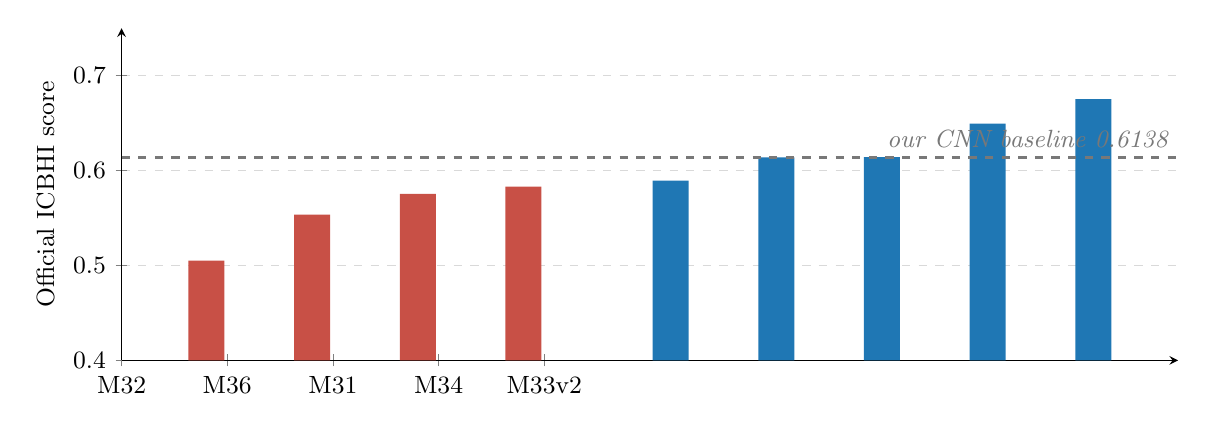
\begin{tikzpicture}
\begin{axis}[
    width=15cm, height=5.8cm,
    ybar, bar width=13pt,
    ymin=0.40, ymax=0.75,
    ylabel={Official ICBHI score}, ylabel style={font=\small},
    symbolic x coords={M32,M36,M31,M34,M33v2,M3,M2,M1,M22,M37,M35},
    xtick=data,
    x tick label style={font=\small}, y tick label style={font=\small},
    ymajorgrids=true, grid style={dashed, gray!30},
    enlarge x limits=0.06, axis lines=left,
]
\addplot[ybar, draw=none, fill=bad, mark=none] coordinates {
    (M32,0.4733) (M36,0.5052) (M31,0.5535) (M34,0.5754) (M33v2,0.5832) };
\addplot[ybar, draw=none, fill=good, mark=none] coordinates {
    (M3,0.5895) (M2,0.6138) (M1,0.6143) (M22,0.6495) (M37,0.6753) (M35,0.6864) };
\draw[thick, dashed, rule] (axis cs:M32,0.6138) -- (axis cs:M35,0.6138)
    node[above left, font=\small\itshape, color=rule] {our CNN baseline 0.6138};
\end{axis}
\end{tikzpicture}
\end{center}

\note{Red bars are the techniques that made things worse. Blue bars held or improved.}

\section*{3. The core idea did not work}

Our disagreement mechanism scored \textbf{AUROC 0.5747} at detecting unknown diseases.

We then tested a baseline that needs no training at all. It reads the energy of the
model output and thresholds it. Four lines of code. It scored \textbf{AUROC 0.6466}.

\begin{figure}[h]
\centering
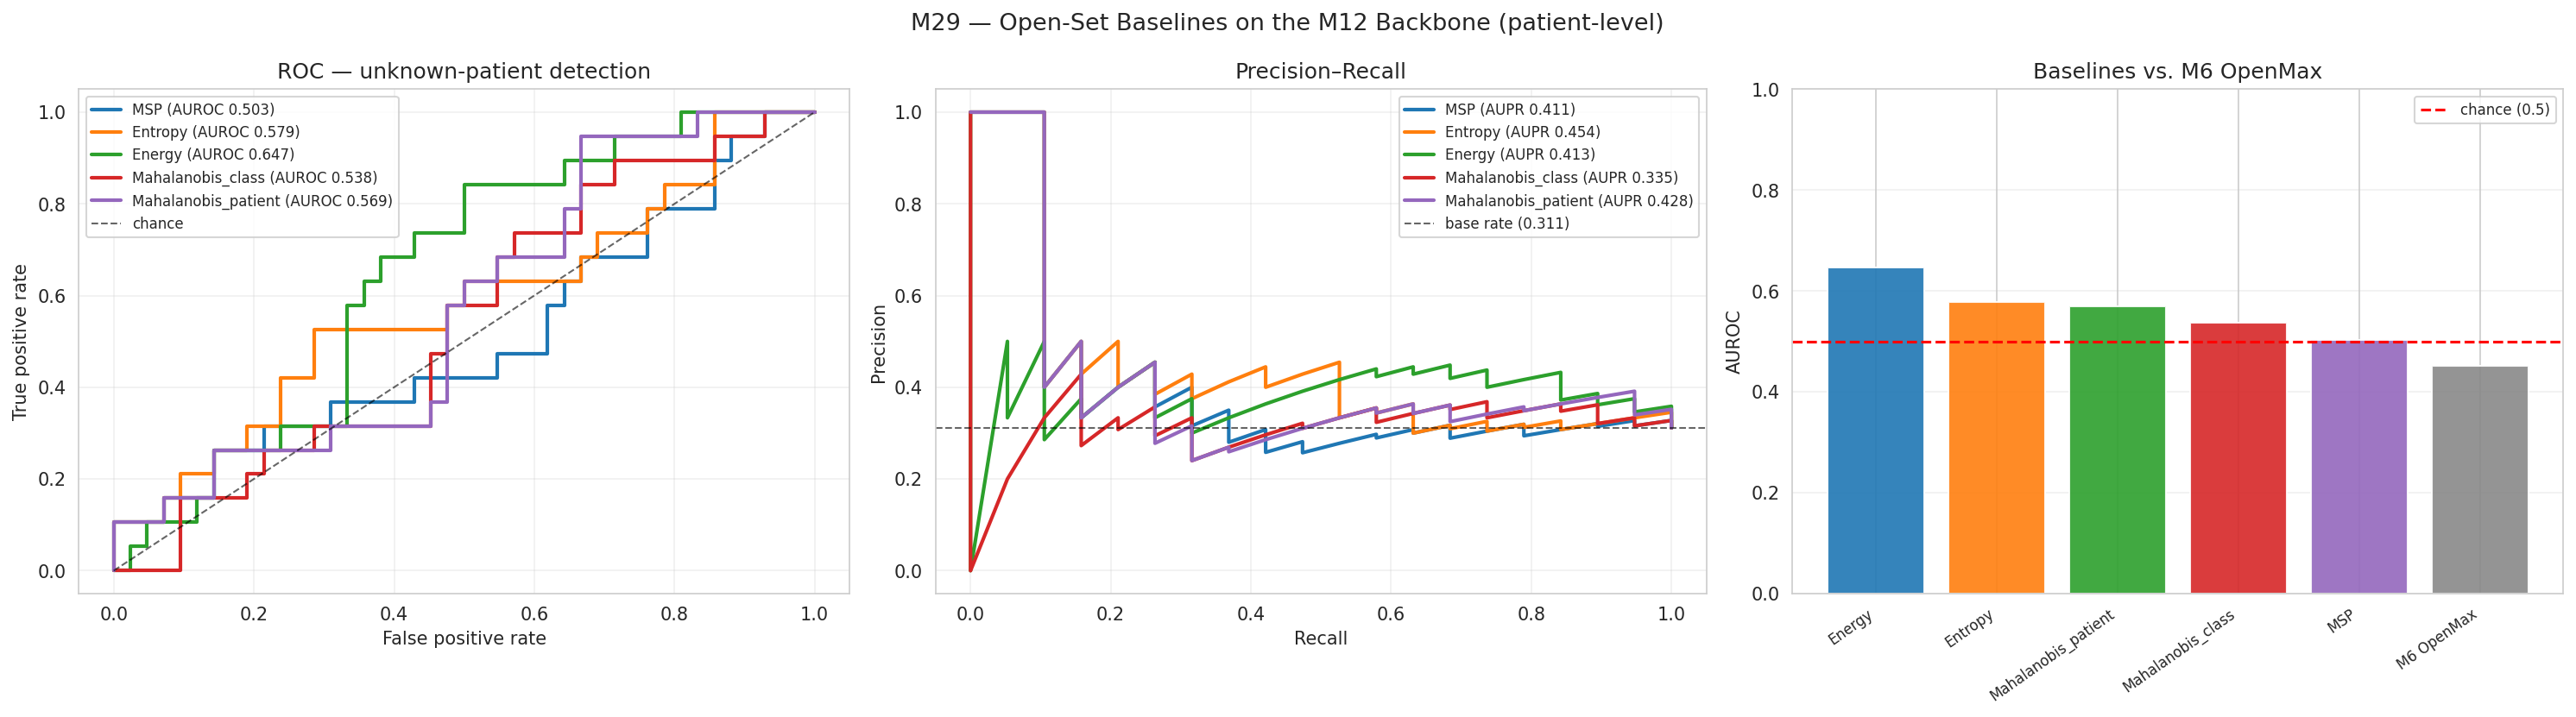
\includegraphics[width=\textwidth]{openset_baselines.png}
\caption{Unknown disease detection on 19 held out patients. The right panel is the
summary. Energy, which needs no training, is the tallest bar. Our OpenMax baseline (M6)
is the lowest and sits below chance.}
\end{figure}

We are not going to try to rescue this mechanism. We already know why it fails. When the
two heads are trained together they learn to agree, so there is no disagreement left to
measure. When trained separately, the disease head becomes a copy of the sound head.

\section*{4. But the honest reading is worse than that}

We computed confidence intervals for every detector. Almost all of them include chance.

\begin{figure}[h]
\centering
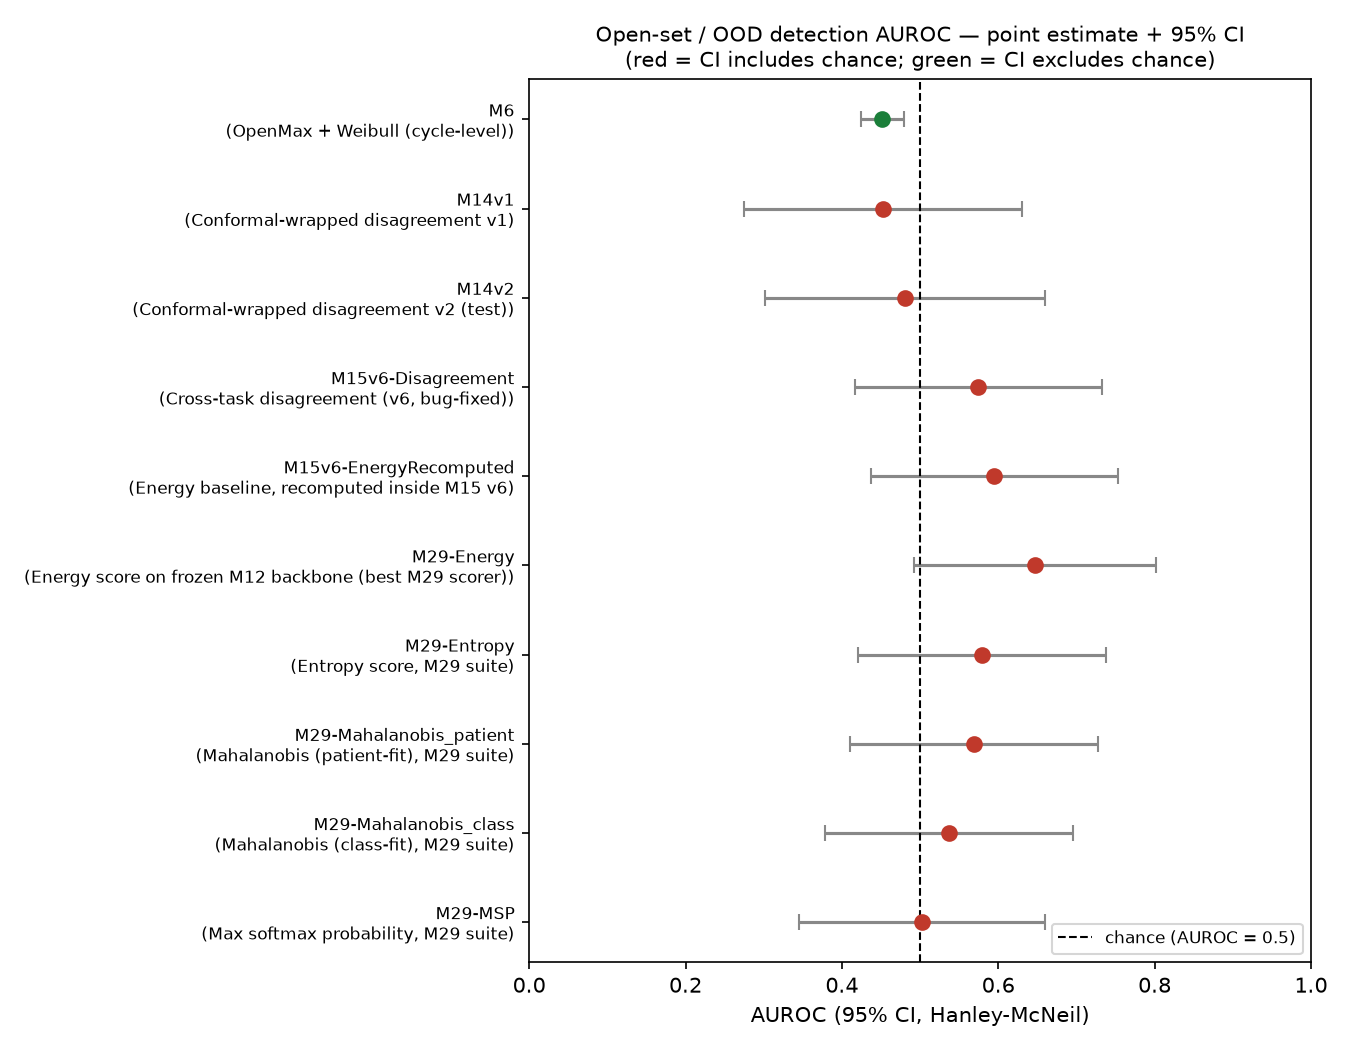
\includegraphics[width=0.86\textwidth]{auroc_forest.png}
\caption{Every open set detector we built, with 95\% confidence intervals. Red means the
interval crosses 0.5, so the result cannot be separated from a coin flip. Only M6 is
clearly different from chance, and it is worse than chance.}
\end{figure}

So the correct statement is not ``our method lost to the baseline''. It is
\textbf{none of these methods has been shown to work at all} on 19 patients. The dataset
does not have enough rare disease cases to tell them apart. No amount of model design
fixes that.

\newpage

\section*{5. Accuracy is capped too}

Our best model, M35, reaches 0.6864. Its training behaviour shows why we do not expect
much more.

\begin{figure}[h]
\centering
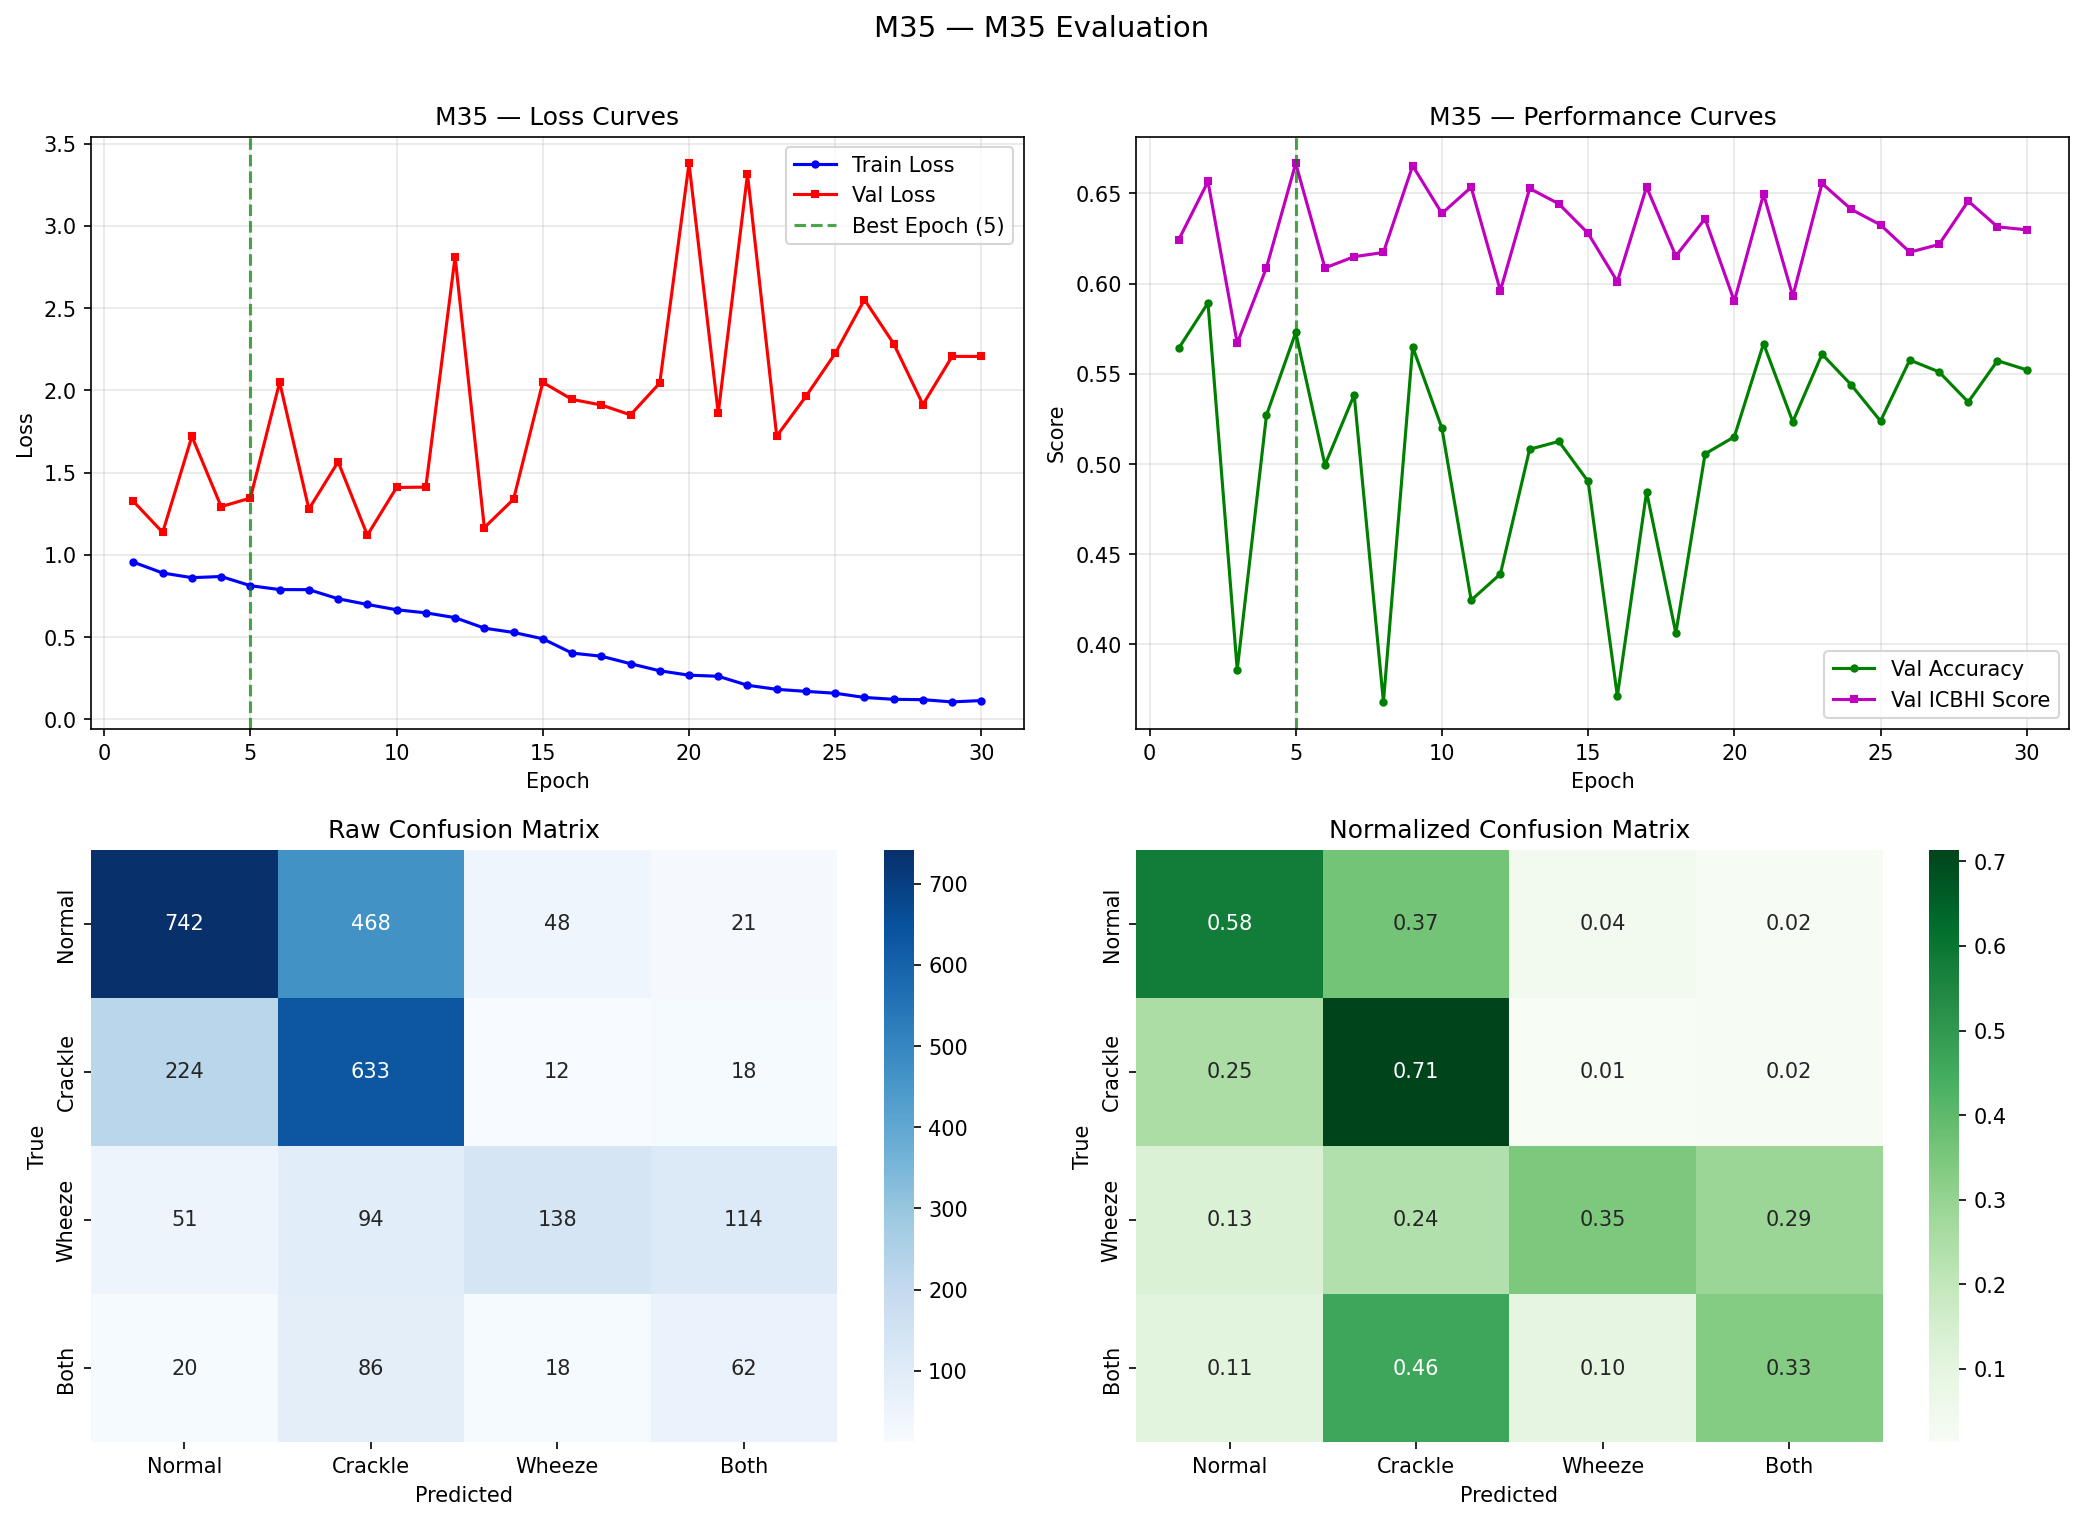
\includegraphics[width=0.92\textwidth]{m35_results.png}
\caption{M35, our best model. Top left: validation loss climbs from epoch 5 onward while
training loss keeps falling, so the model memorises quickly. Best epoch is 5 out of 30.
Bottom right: Wheeze is correct 35\% of the time and Both 33\%. Crackle and Normal are
fine, the rare classes are not.}
\end{figure}

Six of the eight architecture changes we tried made results worse. The two that helped,
physics loss and LoRA, gained about 0.07 over the plain CNN. We are already at the level
of the published literature. Adding a ninth technique will not change this.

\section*{6. A problem we found in our own work}

While auditing the pipeline this month we found that our backbone models reported a
train and test split of ``official 60/40'' in their results files, but had actually used
a fallback rule.

The cause was one wrong capital letter. The code looked for
\texttt{ICBHI\_Challenge\_train\_test.txt}. The real file is
\texttt{ICBHI\_challenge\_train\_test.txt}. On Linux that lookup fails silently, so the
code used a default rule and reported the intended split anyway.

\begin{center}
\begin{tabular}{@{}lcc@{}}
\toprule
 & \textbf{What was reported} & \textbf{The real official split} \\
\midrule
Training patients & 115 & 77 \\
Test patients     & 11  & 49 \\
Test cycles       & 492 & about 2,750 \\
\bottomrule
\end{tabular}
\end{center}

\vspace{4pt}
It is fixed. The split file is now required, its contents are checked against the known
official counts, and the code stops with an error instead of guessing. M2 and M3 are
being retrained and we expect the scores to move.

We are reporting this because we would rather find it ourselves than have a reviewer
find it.

\newpage

\section*{7. What we are doing next}

We are moving from ``make it more accurate'' to ``make it trustworthy and checkable''.

Instead of the model going straight from sound to diagnosis, we force it through a layer
of named clinical sounds.

\vspace{4pt}
\begin{center}
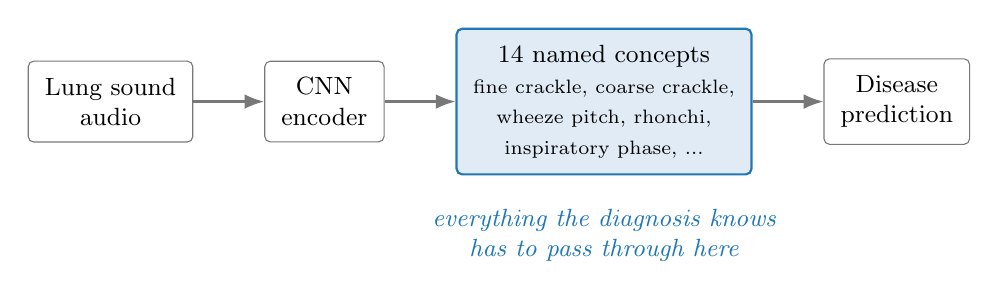
\begin{tikzpicture}[
    box/.style={rectangle, rounded corners=2pt, draw=rule, fill=white,
                minimum height=1.0cm, align=center, font=\small, inner sep=6pt},
    cbox/.style={box, fill=band, draw=good, thick},
    ar/.style={-{Latex[length=2.5mm]}, draw=rule, thick}
]
\node[box] (a) {Lung sound\\audio};
\node[box, right=0.9cm of a] (b) {CNN\\encoder};
\node[cbox, right=0.9cm of b] (c) {14 named concepts\\
    \scriptsize fine crackle, coarse crackle,\\
    \scriptsize wheeze pitch, rhonchi,\\
    \scriptsize inspiratory phase, ...};
\node[box, right=0.9cm of c] (d) {Disease\\prediction};
\draw[ar] (a) -- (b); \draw[ar] (b) -- (c); \draw[ar] (c) -- (d);
\node[below=0.3cm of c, font=\small\itshape, color=good, align=center]
    {everything the diagnosis knows\\has to pass through here};
\end{tikzpicture}
\end{center}

\vspace{4pt}
The concepts come from the physics of the signal. A crackle is a short burst, so we
measure peak to average power. A wheeze is a tone, so we measure spectral flatness and
find the dominant frequency. No manual labelling is needed.

This gives us three things a normal model cannot do.

\begin{enumerate}\setlength{\itemsep}{2pt}
\item \textbf{The model explains itself in clinical words.} It cannot say ``COPD because
      of filter 47''. It has to say ``COPD because coarse crackles at this rate''.
\item \textbf{We can check whether it is telling the truth.} Recent explainable
      respiratory papers claim their models listen to the right frequencies but never
      test it. We measure whether the diagnosis really depends on the concepts, or is
      sneaking information around them.
\item \textbf{A doctor can correct it.} If the model hears a crackle that is not there,
      the doctor overwrites that one value and the diagnosis updates.
\end{enumerate}

\subsection*{Does the code work?}

We wrote the concept extractors and tested them on signals where we know the answer.

\begin{center}
\begin{tabular}{@{}lcccc@{}}
\toprule
\textbf{Test signal} & \textbf{Crackle} & \textbf{Wheeze} & \textbf{Detected freq.} & \textbf{Peak/avg power} \\
\midrule
Noise only    & 0.00  & 0.0 & none   & 11.8 dB \\
400 Hz tone   & 0.00  & 1.0 & 398 Hz & 3.7 dB \\
Short bursts  & 0.996 & 0.0 & none   & 26.9 dB \\
\bottomrule
\end{tabular}
\end{center}

\vspace{4pt}
It finds the tone to within 2 Hz and separates bursts from tones cleanly. The physics is
right on clean signals. Whether it survives real recordings with heartbeat and room
noise is the first thing we test, in week 2.

\subsection*{One test we already know will be interesting}

We compared ICBHI against a pediatric dataset in feature space.

\begin{figure}[h]
\centering
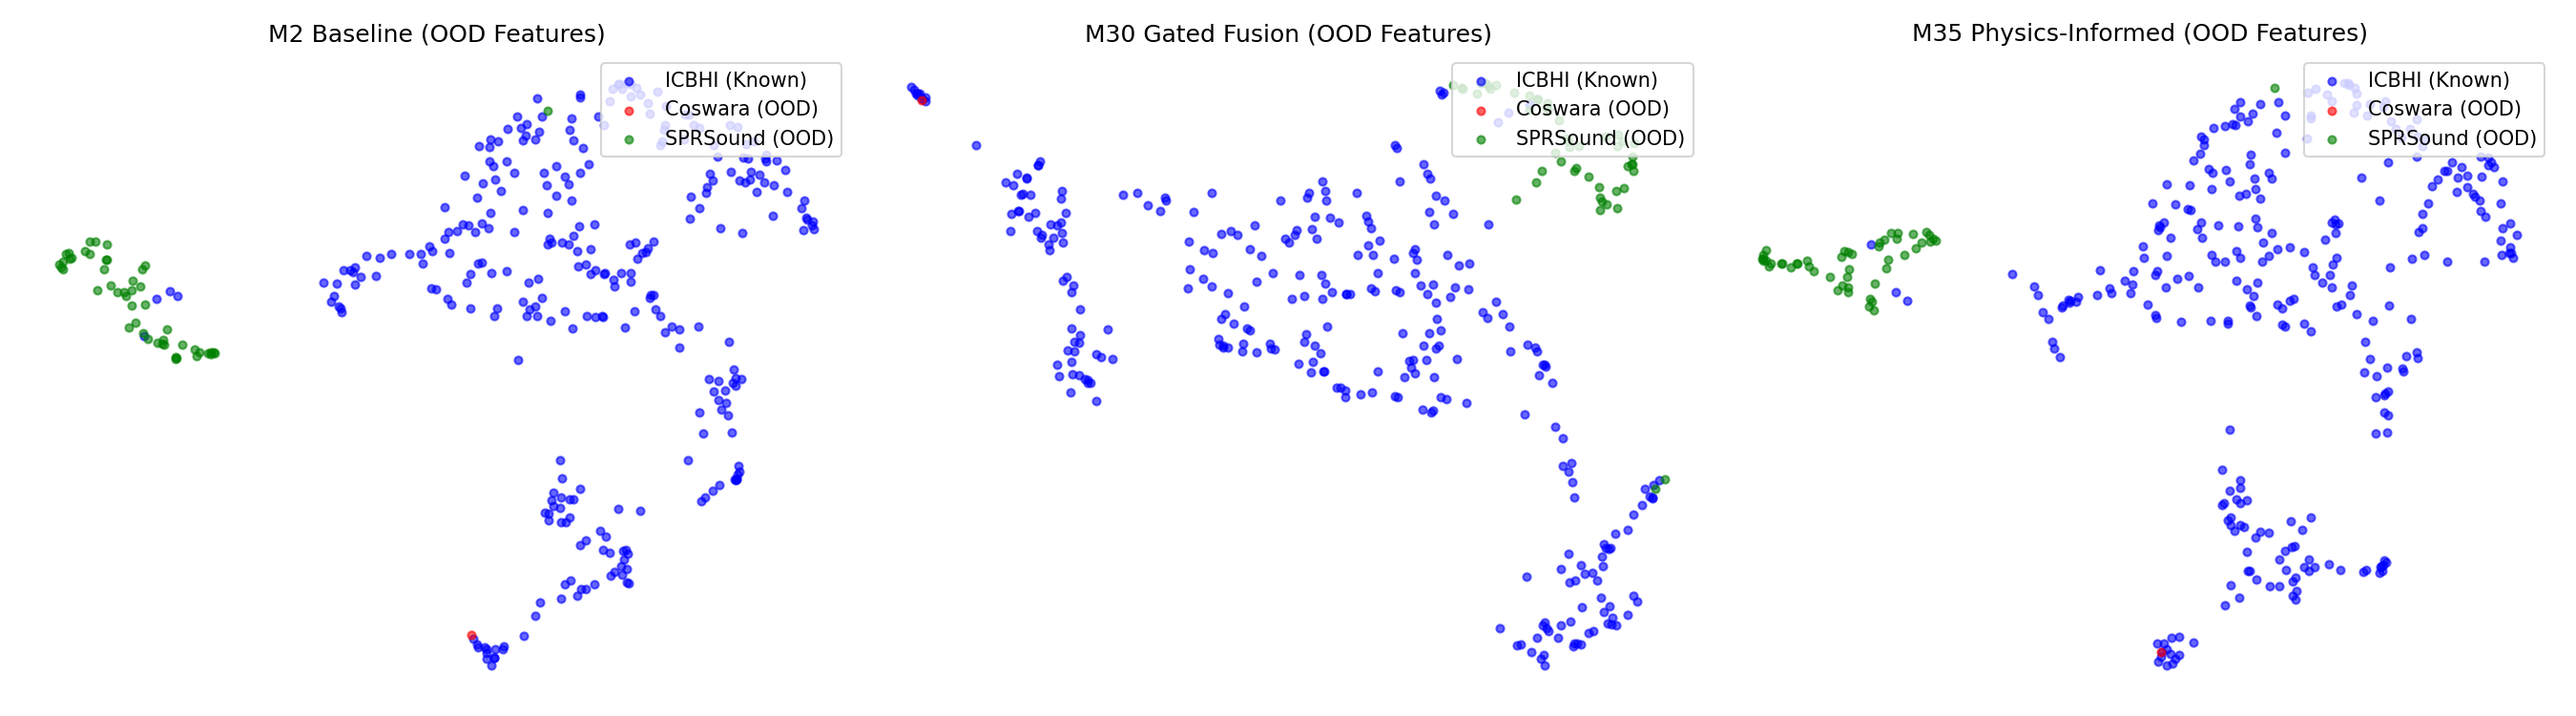
\includegraphics[width=\textwidth]{umap_ood.png}
\caption{Blue is adult ICBHI, green is pediatric SPRSound, across three of our models.
The pediatric data forms its own cluster every time. Children's airways are smaller, so
the sounds sit at different frequencies. This is why we will test whether our
adult tuned concept thresholds still hold on children.}
\end{figure}

\newpage

\section*{8. The plan}

\begin{center}
\begin{tabular}{@{}cll@{}}
\toprule
\textbf{Week} & \textbf{What we do} & \textbf{Output} \\
\midrule
1 to 2 & Extract concepts, check against ICBHI labels & Does the physics hold on real audio \\
3      & Train bottleneck plus three control models   & Accuracy cost of the bottleneck \\
4      & Measure leakage, run the doctor correction   & Two more numbers \\
\textbf{5} & \textbf{Decision point} & \textbf{Which paper we write} \\
6 to 7 & Unknown disease detection, pediatric test, calibration & Full results \\
8      & Figures, statistics, confidence intervals    & Final tables \\
9      & Write the draft                              & Paper \\
\bottomrule
\end{tabular}
\end{center}

\subsection*{Week 5 is the important one}

We are not choosing the conclusion in advance. We read three numbers and the data
decides.

\vspace{4pt}
\begin{center}
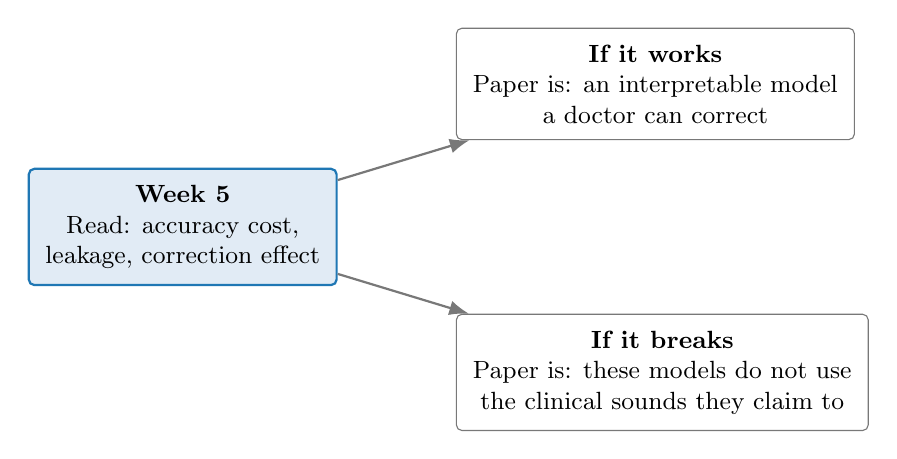
\begin{tikzpicture}[
    box/.style={rectangle, rounded corners=2pt, draw=rule, fill=white,
                align=center, font=\small, inner sep=6pt},
    gate/.style={box, fill=band, draw=good, thick},
    ar/.style={-{Latex[length=2.5mm]}, draw=rule, thick}
]
\node[gate] (g) {\textbf{Week 5}\\Read: accuracy cost,\\leakage, correction effect};
\node[box, above right=0.35cm and 1.5cm of g] (a)
    {\textbf{If it works}\\Paper is: an interpretable model\\a doctor can correct};
\node[box, below right=0.35cm and 1.5cm of g] (b)
    {\textbf{If it breaks}\\Paper is: these models do not use\\the clinical sounds they claim to};
\draw[ar] (g) -- (a); \draw[ar] (g) -- (b);
\end{tikzpicture}
\end{center}

\vspace{4pt}
Both outcomes are publishable. If the bottleneck collapses, that failure is the finding,
and nobody in this field has reported it. This is the main reason we picked this
direction over another accuracy attempt.

\section*{9. What we need from you}

\textbf{One decision.} Should we hand label a small set of cycles, roughly 150 to 300,
for fine grained concepts such as fine versus coarse crackle and breathing phase?

\begin{center}
\begin{tabular}{@{}lll@{}}
\toprule
 & \textbf{Effort} & \textbf{Where it can be published} \\
\midrule
No labelling   & none, we start now      & Good domain journal \\
With labelling & 2 to 3 weeks, in parallel & Q1, the labels become a released dataset \\
\bottomrule
\end{tabular}
\end{center}

\vspace{4pt}
This is the only choice that changes our ceiling. Everything else in the plan runs the
same either way. We would also like to know whether you can point us to a clinician who
could check a sample of the labels.

\vspace{10pt}
\hrule
\vspace{4pt}
\note{Every number here comes from a committed results file with a confusion matrix.
Results we could not verify have been removed, including an earlier 0.8213 that turned
out to use a different train and test split.}

\end{document}
